\section{Upper Limit of Bright FRBs} \label{sec:rate}

We can constrain the upper limit on FRBs at least as bright as our detection threshold by estimating the number of detections over some time as a Poissonian process.
This process has a probability distribution of
\begin{equation}
    p(k|\lambda,\tau) = \frac{(\lambda\tau)^ke^{-\lambda\tau}}{k!}
\end{equation}
for $k$ events given the event rate $\lambda$ and observation time $\tau$.
If we only consider non-detection after some time $\tau_0$, $p(k=0|\lambda,\tau_0)=e^{-\lambda\tau_0}$.
Now, if we want to estimate this rate, $\lambda$, we can solve for $p(\lambda|k=0,\tau_0)$ via Bayes' theorem assuming a flat prior on $\lambda$ where $p(\lambda)\propto1$ via
\begin{equation}
    p(\lambda|k=0,\tau_0) = \frac{p(k=0|\lambda,\tau_0)p(\lambda)}{p(k=0)}=\frac{e^{-\lambda\tau_0}}{\int_{0}^{\infty}d\lambda e^{-\lambda\tau_0}} = \tau_0 e^{-\lambda\tau_0}.
\end{equation}
This is an exponential distribution with a rate of $\tau_0$.
To compare with the estimate from STARE2, we will only consider the station at OVRO in this analysis.
Given our center-frequency beam solid angle of $\sim1.5\,\text{sr}$ from \autoref{eq:beam_solid_angle}, at any given time the station is sensitive to only 12\% of the sky.
As STARE2 continued to run after FRB 200428 until it was superseded by GReX, a station at OVRO has been observing for about five years.
If we assume an observational duty cycle of 75\%, this implies a time on sky of $\tau_0 = 5\times0.12\times0.75 = 0.45\,\text{sky yr}$, in which we observed zero events.
We can repeat this analysis for STARE2's detection, with $k=1$ after time on sky of $\tau_1$.
\begin{equation}
    p(\lambda|k=1,\tau_1) = \frac{p(k=1|\lambda,\tau_1)p(\lambda)}{p(k=1)}=\frac{\lambda\tau_1e^{-\lambda\tau_1}}{\int_{0}^{\infty}d\lambda \lambda\tau_1e^{-\lambda\tau_1}} = \tau_1^2\lambda e^{-\lambda\tau_1}.
    \label{eq:stare_p}
\end{equation}
This is a gamma distribution with a scale of 2 and a rate of $\tau_1$.
We can assume the same observational duty cycle of 75\% over the 448 days before the STARE2 event to compute $\tau_1 = 448/364.25 \times0.12\times0.75 = 0.11\,\text{sky yr}$.
Finally, as FRB events are independent, we can use the joint probability of the STARE2 detection and GReX non-detection to constrain $\lambda$ even further.
We call $k=0,\tau_0$ as the first observational data $d_1$ and $k=1,\tau_1$ as $d_2$ to find
\begin{equation}
    p(\lambda|d_1,d_2) = (\tau_0+\tau_1)^2\lambda e^{-\lambda(\tau_0+\tau_1)}
\end{equation}
using the result in \autoref{eq:stare_p} and substituting $\tau_1$ for $\tau_1+\tau_0$.
This result gives the probability distribution of rate $\lambda$, which describes the event rate of FRBs brighter than our detection threshold, per sky per year.

\begin{figure}[ht!]
    \centering
    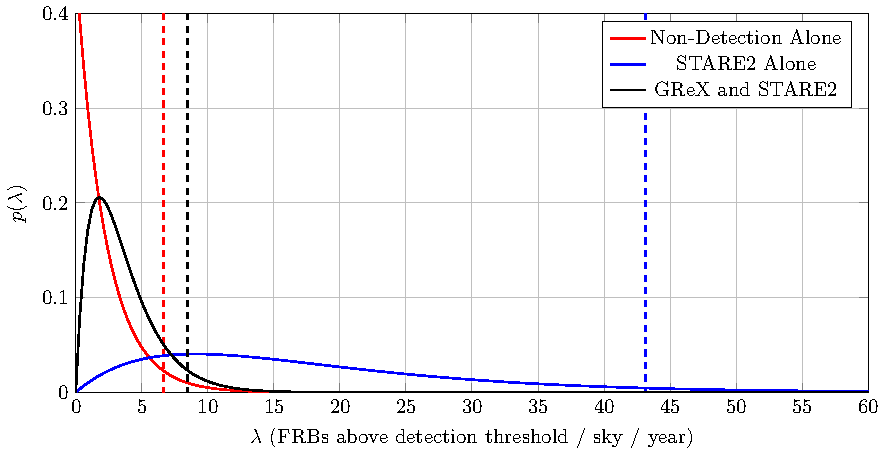
\includegraphics[width=\linewidth]{figures/rate_pdfs.pdf}
    \caption{Probability distribution of FRB rate $\lambda$ with dashed 95\% confidence upper limits}
    \label{fig:rate_pdfs}
\end{figure}

Shown in \autoref{fig:rate_pdfs} are the probability distribution functions for the rate $\lambda$, given the STARE2 detection, the non-detection, and the combined detection and non-detection.
The STARE2 observation placed an upper limit at $43.13\,\text{sky}^{-1}\,\text{yr}^{-1}$ with wide uncertainty due to the limited observation time.
Adding GReX's observation time significantly reduces this estimate to $8.47\,\text{sky}^{-1}\,\text{yr}^{-1}$.
Without including the STARE2 result, the GReX non-detection alone results in a rate estimate of $6.66\,\text{sky}^{-1}\,\text{yr}^{-1}$.
It is important to note that this result only includes the time on sky at OVRO and not any of the other stations.
This additional time for a non-detection would further reduce this upper limit.
A more thorough analysis of the rate including overlapping sky and time, luminosity, etc. will follow in a future paper.

